\chapter{Local Flags}
\label{chap:local_flags}

In the previous chapter we saw how to use flag algebras to bound density functions
asymptotically. Some things are not described by a density function but still feel
"density like" which might lead us to speculate if we can modify the flag algebra method to work
for these functions.

For example, in chapter \ref{chap:pentagon_conjecture} we will see a problem we're calling the
bounded degree Erd\H{o}s' pentagon problem. In approaching that problem we will ask:
"Given a triangle-free graph $G$ with max degree $\Delta(G)$ and some fixed vertex
$v\in V(G)$, how many pentagons (5-cycles) are there containing $v$"?
We want to upper bound this number of pentagons as a function of $\Delta(G)$. The upper
bound of $\Delta(G)^4$ is easily seen, but $\frac{1}{2}\Delta(G)^4$ is also easy to prove.

Phrased differently: If $P(G,v)$ is the number of pentagons in $G$ containing $v$ then
we want to find an asymptotic upper bound on $P(G,v) / \Delta(G)^4$. If we pick a
flag $F=\cfivemarked$ which is a pentagon with a single labelled vertex then this
could be written as $c(F; G^v) / \Delta(G)^4$.

This looks a lot like
a density function, except that our denominator is of the wrong form: It should
be $\in\Theta(|G|^4)$, not $\Delta(G)^4$. It is for this reason that applying classic
flag algebras directly is not promising: Our function is of the wrong form.

It turns out that we can define a new type of "density function" which
can be used to bound functions like $c(F; G^v) / \Delta(G)^4$. These density functions
then also have a rich (but limited) algebraic structure which we can exploit.
In the following sections we introduce our new local density function and then go on to
define local versions of many of the same structures that exist in the classic flag
algebra. We then prove the algebraic structure these \textit{local flags} possess.

\section{Local Flags}

Let $\Gcl$ be some graph class as before.
Let $\Delta$ be some graph parameter $\Delta\colon \Gcl \to \N_0$.

\begin{note}
    We almost exclusively use the maximum degree function $\Delta$ so you can effectively always
    interpret $\Delta(G)$ in this way. In particular all of
    our examples use the max degree function for $\Delta(G)$.
\end{note}

We start by defining the \textit{local density} in the same way as the induced
density (Definition \ref{def:induced_density}) but with a different denominator.
We use the definition of $\sigma$-flags (Definition \ref{def:sigma_flag}) from the
classic flag algebras directly.

\begin{definition}[Local Density]
    Let $(F, \theta), (G,\eta)$ be $\sigma$-flags as before. Then\\
    $c((F,\theta); (G,\eta))$ is
    the induced count (Definition \ref{def:induced_count}). Define the
    \textbf{local density}\\
    $\rho((F, \theta); (G, \eta))$ to be
    \[
        \rho(F; G) := \frac{c(F; G)}{\binom{\Delta(G)}{|F|-|\sigma|}}.
    \]
    Note the $\rho \neq p$ notation.
\end{definition}

Because of our choice of normalisation we are not
guaranteed the $[0,1]$ codomain as in the classic case. In particular this
destroys the nice probabilistic sampling interpretation that we had with the
induced density function. In general this function may be bounded or unbounded:

\begin{example}
    If $\Gcl$ is all graphs then $c(\vertex; G)= |V(G)|$ hence
    $\rho(\vertex; G) = \frac{|G|}{\Delta(G)}$ which is an unbounded function.
\end{example}

\begin{example}
    If $\Gcl$ is all graphs then consider the $\vertex$-flag $\edgemarked$. Then for
    any $G$ with distinguished vertex $v$ we have $c(\edgemarked; G^v)=\deg(v)$
    so $\rho(\edgemarked; G^v) = \frac{\deg v}{\Delta(G)} \leq 1$.
\end{example}

This bounded/unbounded distinction is the key distinction we want to make. Those
flags $F$ with bounded behaviour are those with the exploitable algebraic structure. Indeed
we will eventually define our \textit{local flags} to be those with bounded local density
but we first need to address some technical definitions to avoid pathological cases:

We need a way to technically describe the action of taking a $\sigma$-flag with some
unlabelled vertices and labelling one of those vertices:

\begin{definition}[Label Extension]
    Given a $\sigma$-flag $(F, \theta)$ and some $v\in V(F)$ which is unlabelled
    ($\notin\im\theta$) we can construct a \textbf{label extension}
    $\theta'\colon [|\sigma|+1] \to V(F)$ as
    \[
        \theta'(i) = \begin{cases}
            \theta(i) & \text{if}\ i\in[|\sigma|]\\
            v & \text{otherwise}
        \end{cases}
    \]
    This is an embedding of the type $\sigma'$ obtained by adding new vertex $|\sigma|+1$
    to $\sigma$ such that $\sigma' \cong F[\im \theta \cup \{v\}]$. See figure
    \ref{fig:labelling_ext_example} for an example of a flag and all its possible label
    extensions.
\end{definition}

\begin{figure}[ht]
    \centering
    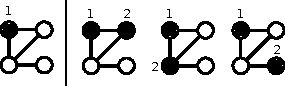
\includegraphics[scale=1.5]{labelling_ext_example.pdf}
    \caption{All possible label extensions of a flag}
    \label{fig:labelling_ext_example}
\end{figure}

The other technicality we need to address is that of the hereditary nature of graph
classes. In the classic flag algebra we always assumed that $\Gcl$ was hereditary. We want
to be able to talk about some non-hereditary graph classes $\Gcl$. This is not a major
obstacle but means we need to adjust our notation.

\begin{definition}[Hereditary Closure]
    Given a graph class $\Gcl$ we define the \textbf{hereditary closure} of $\Gcl$ to be
    the smallest graph class which contains $\Gcl$ and is closed under taking
    induced subgraphs. i.e. it's the graphs $G\in\Gcl$ with their induced subgraphs.

    We denote this as $\HeredG$.
\end{definition}

Now we are ready to define our local flags:

\begin{definition}[Local $\sigma$-Flag]
    \label{def:local_flag}
    Fix some graph class $\Gcl$ and takes its hereditary closure $\HeredG$.
    Let $\sigma$ be a type. Then a $\sigma$-flag $(F, \theta)\in\HeredG{}^\sigma$ is a
    \textbf{local $\sigma$-flag} if we have the following properties:
    \begin{enumerate}
        \item $(G,\eta) \to \rho((F,\theta); (G,\eta))$ is a bounded function as a function
            $\Gcl^\sigma\to\R_{\geq 0}$. (We are very intentionally using $\Gcl$ and not its closure here).
        \item If we label any of $F$'s unlabelled vertices we get another local flag.
    \end{enumerate}
\end{definition}

To state this 2nd property more precisely: We require that for any label extension
$\theta'$ of $\theta$, the induced extended flag $(F,\theta')$ is also a local flag.
This is not a circular definition as any label extension of $(F,\theta)$ reduces the number of
unlabelled vertices
by 1; We could define inductively starting with those flags with no unlabelled vertices.

What we're trying to capture here is that any "subflag" of $F$ is also a local flag, meaning we can
pin down $F$'s vertices and continue to get bounded behaviour.

\begin{example}
    As in the example above $F=\edgemarked$ gives rise to a bounded local
    density function $\rho$. The only label extension of $F$ is the edge
    with both vertices labelled $F' = \edgebothmarked$. This (as with all flags with no
    unlabelled vertices) has $c(F'; G) = 1$ so $\rho(F; G) = 1/\binom{\Delta(G)}{0}=1$
    which is bounded so $F'$ is a local flag. Hence $F=\edgemarked$ is a local flag.
\end{example}

We write $\Glocn^\sigma\subseteq\HeredG{}^\sigma_n$ for the set of local $\sigma$-flags
of size $n$ up to isomorphism, and $\Gloc^\sigma$ for all local $\sigma$-flags. As usual we
can drop the $\sigma$ superscript if $\sigma=\emptyset$.

\begin{note}
    For $\sigma$-flag $F$ the requirement that $\rho(F; G)$ is a bounded function
    is equivalent to requiring that $c(F; G) \in O(\Delta(G)^{|F|-|\sigma|})$.
\end{note}

Comparing this section to the classic flag algebra case (section \ref{sec:flag_algebras})
you might expect us to introduce something akin to the chain rule (lemma \ref{lemma:chain_rule}).
Unfortunately no such relation exists in general for local flags. This is the first big
loss when moving to the new framework: Prima facie it's unclear how one can "project"
small flags into the space of larger flags.

\begin{note}
    This second property we require of local flags is not necessarily implied by
    the first which we show now in lemma \ref{lemma:second_prop_required}.
\end{note}

\begin{lemma}
    \label{lemma:second_prop_required}
    There is a class of graphs $\Gcl$ and $\sigma$-flag $F$ such that
    $G \mapsto \rho(F; G)$ is a bounded function $\Gcl^\sigma \to \R$ but $F$ is
    not a local $\sigma$-flag. i.e. $F$ has a labelled extension with unbounded
    density function.
\end{lemma}
\begin{proof}
    Take $\Gcl$ to be the class of 3-vertex-coloured graphs (black, red and blue) $G$
    which have a single red vertex and $\Delta(G)^2$ blue vertices\footnote{Implicitly the
    rest of the vertices are black} such that there are no edges between red and blue
    vertices.

    Then take $\emptyset$-flag $F=\redbluenonedge$. For any $G\in\Gcl$ we have
    $c(F; G) = \Delta(G)^2$ as there is 1 choice for the red vertex and $\Delta(G)^2$
    choices for the blue. Hence $\rho(F;G) = c(F; G) / \binom{\Delta(G)}{2} \leq 2$.
    Consider then the labelled extension $F' =\redbluenonedgemarked$ of type
    $\redvertex$. We have $c(F'; G)=\Delta(G)^2$ again for any
    $G\in\Gcl^\redvertex$ but now $\rho(F'; G) = \Delta(G)^2 / \Delta(G) = \Delta(G)$ which
    is an unbounded function. Hence $F'$ is not a local $\redvertex$-flag
    meaning $F$ is not a local $\emptyset$-flag.
\end{proof}

Intuitively $F$ is a local $\sigma$-flag (relative to our choice of $\Gcl$ and
$\Delta$) if $\Delta(G)$ bounds the "degree of freedom" for the possible mapping
of $F$'s unlabelled vertices.

\begin{lemma}
    \label{lemma:local_if_connected}
    If $\Delta(G)$ is the max degree function then any $\sigma$-flag $F$ is a
    local $\sigma$-flag if all connected components of $F$ contains a labelled
    vertex.
\end{lemma}

\begin{proof}
    Intuitively the labelled vertices are fixed. The vertices directly connected to
    labelled vertices have $\Delta(G)$ choices. After mapping those we again have
    $\Delta(G)$ choices for their unmapped neighbours etc leading to a total
    bound of $O(\Delta(G)^{|F|-|\sigma|})$ choices.

    The full details of the proof can be found in the proof of
    lemma \ref{lemma:pentagon_local_flags}.
\end{proof}

\section{Algebraic Structure}

Now that we have described local $\sigma$-flags $\Gloc^\sigma$ we can describe their
algebraic structure. Ideally we would like to construct a product structure
on $\Gloc^\sigma$ such that we get a result like theorem \ref{thm:classic_product_lim} but for
the local density function $\rho$. In fact this is exactly what we get: An algebraic structure such
that $\rho(f; G)\rho(g;G) = \rho(f\cdot g; G) + o(1)$ (Theorem \ref{thm:local_product_lim}).

First we take the concept of limit functionals (section \ref{sec:limit_functionals})
from the classic flag algebras with some minor modifications:
First, we require now that a sequence of graphs $(G_k)_{k\in\N}$ is $\Delta$-increasing:
\begin{definition}
    A sequence $(G_k)_{k\in\N}$ is $\Delta$-increasing if the sequence
    $(\Delta(G))_{k\in\N}$ is strictly increasing\footnote{We required that the codomain of
    $\Delta$ was $\N$ so strictly increasing implies unbounded. Generalising $\Delta$
    to a function with codomain $\R$ is likely possible so we would need to add the
    unbounded requirement here.}.
\end{definition}
Then given some $\Delta$-increasing sequence of $\sigma$-flags $(G_k)_{k\in\N}$
and some local $\sigma$-flag
$F$ we can look at $\lim_{k\to\infty}\rho(F; G_k)$. As $F$ is a local $\sigma$-flag
$\rho(F; \cdot)$ is bounded so the image is compact. For this reason (again via Tychonoff's theorem)
any sequence of $\sigma$-flags $(G_k)_{k\in\N}$ contains a convergent subsequence meaning
$\lim_{k\to\infty}\rho(F; G_k)$ exists for all $F\in\Gloc^\sigma$.
Hence we can define a limit functional $\phi\colon\Gloc^\sigma\to\R$
from such a convergent sequence $(G_k)_{k\in\N}$ as $\phi(F):=\lim_{k\to\infty}\rho(F; G_k)$.

As with the classic case we can take the space of formal linear combinations of
local flags $\R\Gloc^\sigma$ and linearly extend $\rho$ and $\phi$ to these
spaces. As before we denote the set of all limit functionals on type $\sigma$ by
$\Phi^\sigma$.

\begin{note}
    Unlike in the classic case we will not be quotienting the space $\R\Gloc^\sigma$ by
    a subspace. This is as we do not have an equivalent relation to the chain rule.
    The side effect of this is that there may be vectors $f \in \R\Gloc^\sigma$ which
    are formally non-zero but have $\phi(f) = 0\ \forall\ \phi\in\Phi^\sigma$.
    This doesn't affect the correctness of our arguments, but does mean the semidefinite
    programs will be larger and therefore may take longer to solve.
\end{note}

We now define the product on $\R\Gloc^\sigma$ which will turn it into an algebra.

\begin{definition}[Local Flag Product]
    Let $F, F'\in\Gloc^\sigma$ be given. Let $n=|F|+|F'|-|\sigma|$, the minimum size of
    a flag which can fit $F$ and $F'$. Then we define:
    \[
        F \cdot F' := \sum_{H \in \Glocn^\sigma} p(F, F'; H) \cdot H
    \]
    Note: This is the induced density function $p$, not the local density function $\rho$.
    Extend this product bilinearly to the space $\R\Gloc^\sigma$ to create an algebra
    $\Lcl^\sigma$.
\end{definition}

\begin{note}
    It will be useful in later chapters to refer to the subspace of $\Lcl^\sigma$
    spanned by flags of a fixed size $n$. Call this subspace $\Lcl^\sigma_n$.
\end{note}

This product has the exact limiting behaviour that we need and some nice algebraic
properties:

\begin{theorem}
    \label{thm:local_product_lim}
    For $f, g \in \Lcl^\sigma$ and $\sigma$-flag $G\in\Gcl^\sigma$ we have
    \[\rho(f; G)\rho(g; G) = \rho(f\cdot g; G) + O\left(\frac{1}{\Delta(G)}\right)\]
    and in particular any limit functional $\phi\in\Phi^\sigma$ is an algebra
    homomorphism $\Lcl^\sigma \to \R$.
\end{theorem}

\begin{lemma}
    \label{lemma:local_assoc}
    The algebra $\Lcl^\sigma$ is commutative, associative and unital.
\end{lemma}

We will prove both of these results after first proving a key technical result which makes this
product work:

\begin{theorem}
    Let $F, F' \in \Gloc^\sigma$ be local $\sigma$-flags and $H$ a $\sigma$-flag
    $\in \HeredG^\sigma$
    of size $n=|F|+|F'|-|\sigma|$ such that $p(F, F'; H) > 0$ then $H$ is a local
    $\sigma$-flag.
\end{theorem}

\begin{proof}
    Let $\theta,\theta'$ be the $\sigma$ embeddings for $F, F'$ and $\eta$ the
    $\sigma$-embedding for $H.$
    To prove $H$ is a local flag we first need to show that $\rho(H; \cdot)$ is a bounded function.
    i.e. $(G \mapsto c(H; G)) \in O(\Delta(G)^{|H|-|\sigma|}).$

    As $p(F, F'; H) > 0$ there is some $U, U'\subseteq V(H)$ such that $U\cap U'=\im\eta$ and
    $F \cong H[U] \land F'\cong H[U']$ as $\sigma$ flags. As $|H|=|F|+|F'|-|\sigma$ we
    have $U \cup U' = V(H)$.

    Let $(G, \zeta)$ be another $\sigma$-flag. If $c(H; G) = 0$ we're done so assume otherwise and
    let $\im\zeta \subseteq V\subseteq V(G)$ be such that $H \cong G[V]$ as $\sigma$-flags. Let
    $\phi$ be this isomorphism. Then In particular $\phi$ induces an embedding of $U, U'$ into
    $V(G)$ such that $\im\zeta = \phi(U) \cap \phi(U')$ and $G[\phi(U)] \cong F\land G[\phi(U')]
    \cong F'$ as $\sigma$-flags.  Hence any choice of an instance of $H$ in $G$ and choice of
    instances $U, U'$ of $F, F'$ in $H$ gives rise to a pair of instances of $F$ and $F'$ in $G.$
    There are at most some constant number $C$ instances of $F, F'$ in $H$ (as the size of $H$ is
    fixed).

    Note then also that any choice of a pair of instances of $F, F'$ in $G$ can be derived from at
    most 1 instance of $H$, as the size of $H$ was chosen to be the minimum possible such that both
    $F,F'$ fit. If the two instances overlap (outside of the required intersection at $\im\zeta$)
    then they don't correspond to an instance of $H.$ If they don't overlap then their
    union corresponds to a single \textit{possible} instance of $H$.

    In summary each instance of $H$ gives rise to some non-zero but bounded number of pairs of
    instances of $F, F'$ in $G$, and each pair of instances of $F, F'$ is induced by at most
    1 instance of $H.$
    Therefore $c(H; G) \leq \frac{1}{C}\cdot c(F; G)\cdot c(F'; G)$. We use then
    the fact that $F$ and $F'$ are local $\sigma$-flags so $c(F; \cdot)$ and
    $c(F'; \cdot)$ are $\in O(\Delta(G)^{|F|-|\sigma|})$ and $\in O(\Delta(G)^{|F'|-|\sigma|})$
    respectively. Hence their product is
    $\in O(\Delta(G)^{|F|+|F'|-2|\sigma|}) = O(\Delta(G)^{|H|-|\sigma|})$ so
    $c(H; \cdot) \in O(\Delta(G)^{|H|-|\sigma|})$ showing $\rho(H; \cdot)$ is a bounded function as
    required.

    \begin{figure}[!ht]
        \centering
        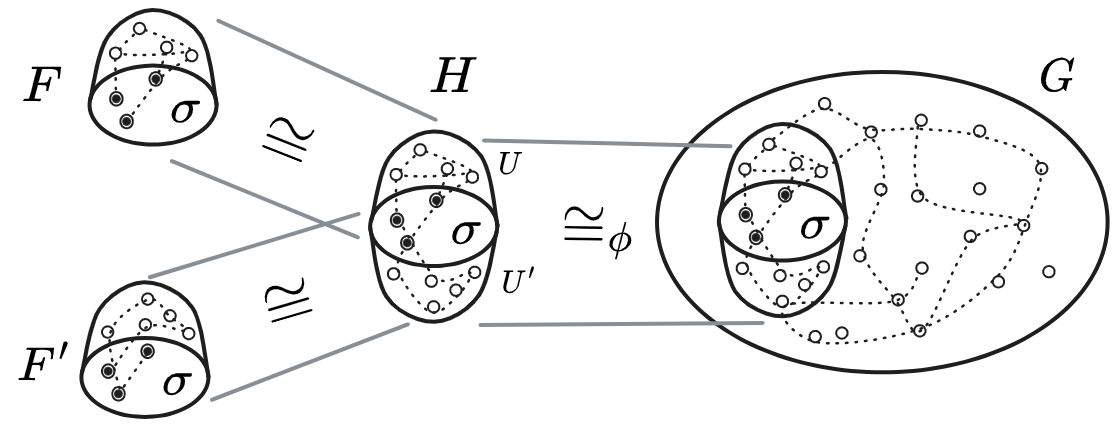
\includegraphics[scale=0.25]{local_flag_product_diagram}
    \end{figure}

    It remains to prove that $H$ still has bounded density after fixing any unlabelled vertices.
    This argument goes almost identically so I just give the high level details. Once again
    pick $U, U' \subseteq V(H)$ where $U\cap U'=\im\eta$ and $F\cong H[U]$ and $F' \cong H[U']$.
    Pick some unlabelled vertex $v\in V(H)\setminus \im\eta$.
    Let $H^v$ be the labelled extension fixing $v$. Then any copy of $H^v$ in $G$ induces
    via $U, U'$ copies of $F, F'$ in $G$. WLOG $v \in U \setminus \im \eta$ so each copy
    of $F$ induced by $U$ is also a copy of $F^v$, the labelled extension of $f$ fixing the
    preimage of $v$. Then as $F$ is local $F^v$ has bounded corresponding density
    function. Once again we have some constant $C$ number of choices for $U, U'$ so we
    get
    $c(H^v; G) \leq \frac{1}{C} c(F^v; G) \cdot c(F'; G) \in
    O(\Delta(G)^{|F|-(|\sigma|+1)+|F'|-|\sigma|}) = O(\Delta(G)^{|H|-(|\sigma|+1)})$
    as required.  $\therefore H$ is a local flag.
\end{proof}

The value of this theorem is that it tells us that our local product definition is
equivalent to summing over all $\sigma$-flags, not just the local flags:

\begin{corollary}
    \label{corollary:local_product}
    For local flags $F, F' \in \Gloc^\sigma$ we have
    \[
        F \cdot_{\Lcl^\sigma} F'
        = \sum_{H\in\Glocn^\sigma}p(F, F'; H)\cdot H
        = \sum_{H\in\HeredG{}_n^\sigma}p(F, F'; H)\cdot H
    \]
    where $n=|F|+|F'|-|\sigma|$.
\end{corollary}

This allows us to prove our product limiting result (Theorem \ref{thm:local_product_lim}).

\begin{proof}[Proof of theorem \ref{thm:local_product_lim}]
    Let $(F,\theta), (F',\theta') \in\Gloc^\sigma$ be local $\sigma$-flags and
    $(G,\eta) \in \Gcl^\sigma$ a
    $\sigma$-flag. We compute
    \[
        \begin{split}
            \rho(F; G)\cdot\rho(F';G) -\rho(F\cdot F'; G)
            &= \rho(F; G)\cdot\rho(F';G)
                - \left(\sum_{H\in\Glocn^\sigma} p(F, F'; H)\rho(H; G) \right)\\
            &= \rho(F; G)\cdot\rho(F';G)
                - \left(\sum_{H\in\HeredG{}_n^\sigma} p(F, F'; H)\rho(H; G) \right)\\
            &= \frac{c(F; G)\cdot c(F';G)}{\binom{\Delta(G)}{|F|-k}\binom{\Delta(G)}{|F'|-k}}
                - \frac{\sum_{H\in\HeredG{}^\sigma_n} c(F, F'; H)c(H; G)}
                {\binom{n-k}{|F|-k}\binom{\Delta(G)}{n-k}}
            \end{split}
    \]
    where $k=|\sigma|$ and $n=|F|+|F'|-k$.
    First we note the denominators are asymptotically equivalent. It is a standard
    binomial identity that
    $\binom{\Delta(G)}{n-k}\binom{n-k}{|F|-k} = \binom{\Delta(G)}{|F|-k}\binom{\Delta(G)-(|F|-k)}{|F'|-k}$
    hence
    \[
        \lim_{\Delta(G)\to\infty}
        \frac{\binom{n-k}{|F|-k}\binom{\Delta(G)}{n-k}}{\binom{\Delta(G)}{|F|-k}\binom{\Delta(G)}{|F'|-k}}
        = \lim_{\Delta(G)\to\infty}
        \frac{\binom{\Delta(G)}{|F'|-k}}{\binom{\Delta(G)-(|F|-k)}{|F'|-k}}
        = 1.
    \]
    Both denominators are asymptotically equivalent and $\in\Omega(\Delta(G)^{n-k})$ so we
    can focus on the numerators:
    \[
        c(F;G)c(F';G) - \sum_{H\in\HeredG{}^\sigma_n}c(F,F';H)c(H;G).
        \tag{$\dagger$}
    \]
    It suffices to show $(\dagger) \in O(\Delta(G)^{n-k-1})$.

    The term $c(F; G)c(F';G)$ counts the number of pairs of subsets
    $\im\eta \subseteq U, U' \subseteq V(G)$ such that $F \cong G[U]$ and $F'\cong G[U']$.
    Comparatively the sum $\sum_{H\in\HeredG{}^\sigma_n} c(F, F'; H)c(H; G)$ counts the number
    of subsets $\im\eta U, U' \in V(G)$ such that $F\cong G[U]$, $F'\cong G[U']$ \textit{and}
    $U \cap U' = \im \eta$. This relies on
    corollary \ref{corollary:local_product}
    which let us sum over all possible flags of size $n$.

    Clearly then ($\dagger$) counts the
    number of pairs of subsets $\im\eta \subseteq U, U' \subseteq V(G)$ such that
    $F \cong G[U], F'\cong G[U']$ and $U \cap U' \neq \im \eta$ meaning there is
    an overlap of the image of the unlabelled vertices of $F, F'$.

    To see intuitively that $(\dagger)\in O(\Delta(G)^{n-k-1})$
    remember that $F,F'$ being local flags means $\Delta(G)$
    bounds the degree of freedom of choosing the image of each of their unlabelled vertices.
    Then $\Delta(G)^{n-k}$ represents the degree
    of freedom of choosing pairs of embeddings of $F, F'$ with no constraints; Adding
    the constraint that the embeddings must overlap means reducing the degree of freedom
    by at least one, giving $\Delta(G)^{n-k-1}$. We show the argument in detail here:

    We calculate an upper bound on ($\dagger$) by summing for each $U$ embedding $F$ into $G$
    and over each unlabelled $v \in V(F)$ the maximum number of $U'$ embeddings of $F'$ which
    overlap on the image of $v$.

    Fix $\im\eta\subseteq U \subseteq V(G)$ such that $F \cong G[U]$ and
    $v\in V(F) \setminus \im\eta$. Call the isomorphism $\phi$. We ask then
    how many $\im\eta \subseteq U' \subseteq V(G)$ are there such that $\phi(v)\in U'$ and
    $F' \cong G[U']$? We can upper bound this by summing over each unlabelled
    $w \in V(F')$ and asking how many $U'$ embeddings are there where the isomorphism
    maps $w$ to $\phi(v)$.
    This is exactly what is answered by taking a labelled extension of $F'$ labelling
    $w$ and extending the label of $G$ to map $w$ to $\phi(v)$. We are guaranteed that
    $F'$ is a local flag so this labelled extension also has bounded density. In particular
    $c((F')^w; G^{\phi(v)})\in O(\Delta(G)^{|F'|-(k+1)})$.

    \begin{figure}[!ht]
        \centering
        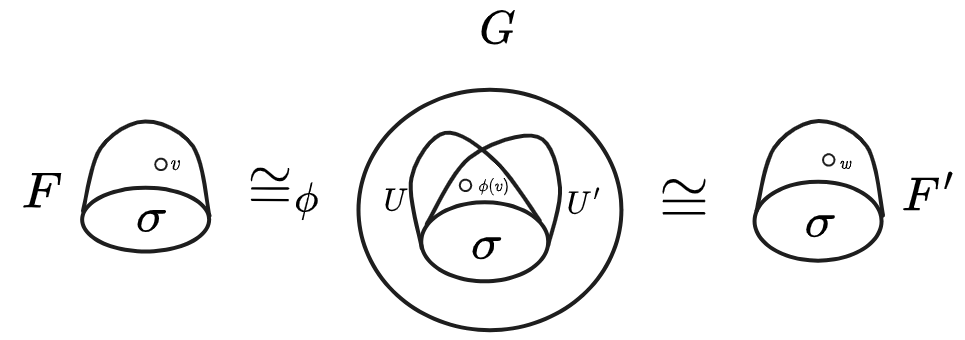
\includegraphics[scale=0.25]{local_flag_limit_diagram}
    \end{figure}

    We have a constant number of choices of $w$ and $v$ and $c(F; G) \in O(\Delta(G)^{|F|-k})$
    choices for $U$ giving us a total upper bound of
    $O(\Delta(G)^{|F|-k + |F'|-(k+1)}) = O(\Delta(G)^{n-k-1})$ as required.
    \[
        \therefore \rho(F; G)\rho(F'; G) - \rho(F\cdot F'; G)
        = \frac{O(\Delta(G)^{n-k-1})}{\Omega(\Delta(G)^{n-k})}
        = O\left(\frac{1}{\Delta(G)}\right).
    \]
    This then extends linearly to $\Lcl^\sigma = \R\Gloc^\sigma$ as
    the vector space only contains finite combinations.
    This has the immediate corollary of showing that any limit functional
    $\phi\in\Phi^\sigma$ is an algebra homomorphism $\Lcl^\sigma \to \R$.
\end{proof}

Finally we can prove lemma \ref{lemma:local_assoc}, showing $\Lcl^\sigma$ to be associative,
commutative and unital.

\begin{proof}[Proof of Lemma \ref{lemma:local_assoc}]
    It is clear by definition that the product is commutative.

    To show associativity let $F_1, F_2, F_3$ be local $\sigma$-flags.
    Then let $k = |\sigma|, \ell = |F_1|+|F_2|-k$ and $n = |F_1|+|F_2|+|F_3|-2k$. Then
    we can calculate:

    \[
        \begin{split}
            (F_1 \cdot F_2) \cdot F_3
            &= \left(\sum_{H\in\Glocsub{\ell}^\sigma} p(F_1,F_2;H)H\right) \cdot F_3\\
            &= \left(\sum_{H\in\HeredG{}\ell^\sigma} p(F_1,F_2;H)H\right) \cdot F_3\\
            &= \sum_{H\in\HeredG{}_\ell^\sigma} p(F_1,F_2;H)(H \cdot F_3)\\
            &= \sum_{H\in\HeredG{}_\ell^\sigma} p(F_1,F_2;H)
                \left(\sum_{G\in\Glocn^\sigma} p(H,F_3;G)G \right)\\
            &= \sum_{G\in\Glocn^\sigma}
                \left(\sum_{H\in\HeredG{}_\ell^\sigma} p(F_1,F_2;H) p(H,F_3;G) \right) G
        \end{split}
    \]
    Then as we used corollary \ref{corollary:local_product} to get a sum over all flags, not just local ones, we can
    apply the chain rule for induced densities (lemma \ref{lemma:chain_rule})
    to get:
    \[
            (F_1 \cdot F_2) \cdot F_3
            = \sum_{G\in\Glocn^\sigma} p(F_1, F_2, F_3; G)\cdot G
    \]
    This is symmetric in all 3 terms so clearly $(F_1\cdot F_2)\cdot F_3 = F_1 \cdot (F_2\cdot F_3)$
    so $\Lcl^\sigma$ is associative.

    Finally take the type $\sigma$ and view it as a $\sigma$-flag implicitly. Then
    $c(\sigma; G)=1$ for any $\sigma$-flag $G$ so $\rho(\sigma; G)=1/\binom{\Delta(G)}{0}=1$
    showing $\sigma$ is a local $\sigma$-flag $\implies \sigma\in\Lcl^\sigma$.
    Then it is easy to see that $\sigma$ is a unit in this algebra as for any
    $F\in\Lcl^\sigma$ we have
    $F\cdot\sigma = \sum_{H \in \Glocsub{|F|}^\sigma}p(F,\sigma; H)H=F$
    as the only flag of size $|F|$ which contains a copy of $F$ is $F$ itself.
\end{proof}

\section{Positivity}

We previously adopted the idea of limit functionals almost directly from the
classic flag algebra, we now do the same with positivity. 
\begin{definition}[Positive Element]
    We say $f\in\Lcl^\sigma$ is a positive element, denoted $f \geq_{\Lcl^\sigma} 0$ or
    just $f\geq 0$, if $\phi(f) \geq 0\ \forall \phi\in\Phi^\sigma$.
\end{definition} 

We then denote the convex cone of all positive elements of $\Lcl^\sigma$ by
$\SemCone^\sigma$. We again call this the (local) semantic cone.

\section{Averaging Local Flags}

So far we have made restrictions no restrictions on what types $\sigma$ we consider, but
it will prove useful to look at only a select set of types we call \textit{local types}.
\begin{definition}[Local Type]
    We say that a type (definition \ref{def:type}) is a \textbf{local type}
    if $\downflag{F}$ is a local $\emptyset$-flag for all $F\in\Gloc^\sigma$.
\end{definition}

We also give a useful equivalent condition:
\begin{lemma}
    \label{lemma:local_type_equiv}
    A type $\sigma$ is a local type iff $\sigma$ is itself a local $\emptyset$-flag
\end{lemma}

\begin{proof}
    One direction is easy to see. If $\sigma$ is a local type then as $\sigma\in\Gloc^\sigma$
    we have $\downflag{\sigma}\in\Gloc^\emptyset$ but $\downflag{\sigma}=\sigma$ so
    $\sigma$ is a local $\emptyset$-flag.

    To show the other direction assume $\sigma$ is itself a local $\emptyset$-flag
    meaning $c(\sigma; G) \in O(\Delta(G)^{|\sigma|})$. Let $(F, \theta) \in\Gloc^\sigma$ be
    given, then we also have\\
    $c((F, \theta); (G, \eta)) \in O(\Delta(G)^{|F|-|\sigma|})$.
    Let $C_\sigma$ be the constant such that\\
    $c(\sigma; G) \leq C_\sigma \Delta(G)^{|\sigma|}\forall G\in\Gcl$ and
    $C_F^\sigma$ the constant such that\\
    $c((F, \theta); (G, \eta)) \leq C_F^\sigma\Delta(G)^{|F|-|\sigma|}\forall
    (G,\eta)\in\Gcl^\sigma$. For fixed $\sigma$ and $U \subseteq V(G)$ there is
    a finite number of possible embeddings $\eta$ such that $(G,\eta)$ is a
    $\sigma$-embedding and $\im\eta=U$, namely the size of the automorphism group of $\sigma$
    $|\mathrm{Aut}(\sigma)|$.

    We want to show that $\downflag{(F,\theta)}=F$ is a local $\emptyset$-flag so first need to show
    $c(F; G) \in O(\Delta(G)^{|F|})$.
    Given any embedding $(G,\eta)$ and $\im\eta \subseteq U \subseteq V(G)$ such that
    $(F,\theta) \cong (G[U],\eta)$ we must have $F \cong G[U]$ as $\emptyset$-graphs.
    This gives us a map into copies of $F$ in $G$ which is just forgetting the labels
    in both $(G,\eta)$ and $(F,\theta)$.
    Conversely consider some copy of $F$ in $G$ $U \subseteq V(G)$ ($F \cong G[U]$ as
    $\emptyset$-flags). Then as $(F,\theta)$ is a $\sigma$-flag there is some $V\subseteq U$ such
    that $\sigma \cong G[V]$. We can then construct a $\sigma$-flag $(G,\eta)$ where
    $\im\eta=V$ such that $(F, \theta) \cong (G[U], \eta)$ as $\sigma$-flags.
    This shows us that the previous map must be surjective.
    Hence
    \[
        \begin{split}
            c(F; G)
            &\leq \left|\{ ((G, \eta), U)\colon
                \im\eta \subseteq U \subseteq V(G)\ \text{such that}\ (F,\theta) \cong (G[U],\eta)
                \}\right|\\
            &\leq \sum_{(G,\eta)\in\Gcl^\sigma}
                \left|\{ U\colon
                \im\eta \subseteq U \subseteq V(G)\ \text{such that}\ (F,\theta) \cong (G[U],\eta)
                \}\right|\\
            &\leq \sum_{(G,\eta)\in\Gcl^\sigma} c((F,\theta), (G,\eta))\\
            &\leq \sum_{(G,\eta)\in\Gcl^\sigma} C_F^\sigma\Delta(G)^{|F|-|\sigma|}\\
            &\leq |\mathrm{Aut}(\sigma)|c(\sigma; G) C_F^\sigma\Delta(G)^{|F|-|\sigma|}\\
            &\leq |\mathrm{Aut}(\sigma)|C_\sigma\Delta(G)^{|\sigma|} C_F^\sigma\Delta(G)^{|F|-|\sigma|}\\
            &\in O(\Delta(G)^{|F|})
        \end{split}
    \]
    as required. It remains to show that any labelled extension of $\downflag{F}$
    also has bounded density function. $\downflag{F}$ is an $\emptyset$-flag so
    a labelled extension $F'$ of $\downflag{F}$ is just $F$ with a single labelled vertex.
    There are 2 cases but they both proceed similarly. If this labelled
    vertex is in $\im\theta\subseteq V(F)$ then as $\sigma$ is a local $\emptyset$-flag
    by an almost identical argument to the previous we get a bound of
    $c(F'; G^v) \in O(\Delta(G)^{|F|-1})$. The other case is that the newly labelled
    vertex of $\downflag{F}$ is one of the unlabelled vertices in $F$, in which case
    we use that $F$ is a local $\sigma$-flag to again bound
    $c(F'; G^v) \in O(\Delta(G)^{|F|-1})$ as required.
    Therefore $\downflag{F}$ is a local $\emptyset$-flag.
\end{proof}

We adopt this definition of local type because we would like to introduce an averaging
operator $\llbracket \cdot \rrbracket \colon \Lcl^\sigma \to \Lcl^\emptyset$ akin
to definition \ref{def:classic_averaging} but we cannot just apply this map directly
as we don't generally have a guarantee that $\llbracket f \rrbracket \in \Lcl^\emptyset$ even
if $f\in\Lcl^\sigma$. By our definition above this map is well
defined if $\sigma$ is local type.

\begin{definition}[Averaging operator]
    As a reminder we have a normalisation function $q_\sigma\colon\Gcl^\sigma\to[0, 1]$
    given in definition \ref{def:averaging_normalisation}.
    Define the \textbf{averaging operator}
    $\llbracket \cdot \rrbracket\colon \R\Gcl^\sigma \to \R\Gcl^\emptyset$
    as before by defining
    $\llbracket F \rrbracket = q_\sigma(F)\downflag{F}$ for $F\in\Gcl^\sigma$ and
    extend linearly.

    If $\sigma$ is a local type and we restrict the domain to $\R\Gloc^\sigma = \Lcl^\sigma$
    we get a map
    $\llbracket \cdot\rrbracket\colon \Lcl^\sigma \to \Lcl^\emptyset$.
\end{definition}

We have a very nice result (lemma \ref{lemma:classic_exp_flags}) in the classic case where this
operator represents an average in a very concrete way:
$\E_\theta[p(F; (G,\theta))] = \frac{p(\llbracket F \rrbracket; G)}{p(\llbracket\sigma\rrbracket;
G)}$
We do not get quite such a neat relation for local densities, but we do get the relation
in the limit:

\begin{lemma}
    \label{lemma:local_averaging_exp}
    For $\sigma$-flag $F$ and graph ($\emptyset$-flag) $G\in\Gcl$ we have
    \[
        \E_\theta[\rho(F; (G,\theta))] \sim
        \frac{\rho(\llbracket F\rrbracket; G)}{\rho(\llbracket \sigma\rrbracket; G)}
        \ \text{as}\ \Delta(G) \to \infty
    \]
    where $\theta$ is a uniformly random $\sigma$-embedding into $G$.
\end{lemma}

\begin{proof}
    This proof uses the fact that this relation holds for induced densities
    (lemma \ref{lemma:classic_exp_flags}) and the following relation between
    induced and local densities:
    For any $\sigma$-flags $H$ and $G$ we have
    \[
        \rho(H; G)
        = \frac{c(H; G)}{\binom{\Delta(G)}{|H|-|\sigma|}}
        = \frac{\binom{|G|-|\sigma|}{|H|-|\sigma|}c(H;
        G)}{\binom{|G|-|\sigma|}{|H|-|\sigma|}\binom{\Delta(G)}{|H|-|\sigma|}}
        =
        \frac{\binom{|G|-|\sigma|}{|H|-|\sigma|}}{\binom{\Delta(G)}{|H|-|\sigma|}}\frac{c(H;G)}{\binom{|G|-|\sigma|}{|H|-|\sigma|}}
        = \frac{\binom{|G|-|\sigma|}{|H|-|\sigma|}}{\binom{\Delta(G)}{|H|-|\sigma|}}p(H;G)
    \]
    Therefore
    \[
        \frac{\rho(\llbracket F\rrbracket; G)}
        {\rho(\llbracket \sigma\rrbracket; G)}
        =
        \frac{p(\llbracket F\rrbracket; G)}
        {p(\llbracket \sigma\rrbracket; G)}
        \frac{\binom{|G|}{|F|}}{\binom{\Delta(G)}{|F|}}
        \frac{\binom{\Delta(G)}{|\sigma|}}{\binom{|G|}{|\sigma|}}.
    \]
    Now we use lemma \ref{lemma:classic_exp_flags} to show
    \[
        \begin{split}
            \frac{\rho(\llbracket F\rrbracket; G)}
            {\rho(\llbracket \sigma\rrbracket; G)}
            &= \E_\theta[p(F; (G,\theta))]
            \frac{\binom{|G|}{|F|}}{\binom{\Delta(G)}{|F|}}
            \frac{\binom{\Delta(G)}{|\sigma|}}{\binom{|G|}{|\sigma|}}\\
            &= \E_\theta[\rho(F; (G,\theta))]
            \frac{\binom{\Delta(G)}{|F|-|\sigma|}}{\binom{|G|-|\sigma|}{|F|-|\sigma|}}
            \frac{\binom{|G|}{|F|}}{\binom{\Delta(G)}{|F|}}
            \frac{\binom{\Delta(G)}{|\sigma|}}{\binom{|G|}{|\sigma|}}\\
            &= \E_\theta[\rho(F; (G,\theta))]
            \frac{\binom{\Delta(G)}{|F|-|\sigma|}\binom{\Delta(G)}{|\sigma|}}
            {\binom{\Delta(G)}{|F|}}
            \frac{\binom{|G|}{|F|}}
            {\binom{|G|-|\sigma|}{|F|-|\sigma|}\binom{|G|}{|\sigma|}}
        \end{split}
    \]
    We can use standard binomial relations to reduce this to
    \[
        \frac{\rho(\llbracket F\rrbracket; G)}
        {\rho(\llbracket \sigma\rrbracket; G)}
        = \E_\theta[\rho(F; (G,\theta))]
        \frac{\binom{\Delta(G)}{|F|-|\sigma|}\binom{\Delta(G)}{|\sigma|}}
        {\binom{\Delta(G)}{|F|}\binom{|F|}{|\sigma|}}
        = \E_\theta[\rho(F; (G,\theta))]
        \frac{\binom{\Delta(G)}{|F|-|\sigma|}}
        {\binom{\Delta(G)-|\sigma|}{|F|-|\sigma|}}
    \]
    Then
    $\lim_{\Delta(G)\to\infty}\binom{\Delta(G)}{|F|-|\sigma|}/\binom{\Delta(G)-|\sigma|}{|F|-|\sigma|}
    = 1$ so we do indeed get
    \[
        \frac{\rho(\llbracket F\rrbracket; G)}
        {\rho(\llbracket \sigma\rrbracket; G)}
        = (1+o(1)) \E_\theta[\rho(F; (G,\theta))]
        \implies
        \frac{\rho(\llbracket F\rrbracket; G)}
        {\rho(\llbracket \sigma\rrbracket; G)}
        \sim \E_\theta[\rho(F; (G,\theta))].
    \]
\end{proof}

Now we can show that the averaging operator preserves positivity as in the
classic case (lemma \ref{lemma:classic_pos_preserve}). We only get this
behaviour if $\sigma$ is a local type.

\begin{lemma}
    \label{lemma:local_pos_preserve}
    Let $\sigma$ be a local type. Then the averaging operator preserves positive
    elements of $\Lcl^\sigma$:
    $\llbracket \SemCone^\sigma \rrbracket \subseteq  \SemCone^\emptyset$.
    In particular as with the classic case we have $\llbracket f^2 \rrbracket \geq 0$
    for all $f\in\Lcl^\sigma$.
\end{lemma}

\begin{proof}
    As $\sigma$ is a local type we have that
    $\llbracket \SemCone^\sigma \rrbracket \subseteq \Lcl^\emptyset$.

    Let $f\in\SemCone^\sigma$ be given and assume for sake of contradiction that
    $\llbracket f \rrbracket \notin\SemCone^\emptyset$. Then there must exist
    some limit functional $\phi\in\Phi^\emptyset$ such that $\phi(f)<0$. Equivalently
    there is some $\Delta$-convergent sequence of graphs $(G_k)_{k\in\N}$
    such that $\lim_{k\to\infty}\rho(f; G_k) < 0$.

    By lemma \ref{lemma:local_averaging_exp} we know that
    \[
        \rho(\llbracket f\rrbracket; G_k) = (1+o(1)) \rho(\llbracket \sigma \rrbracket; G_k)
        \E_\theta[\rho(f; (G_k,\theta))]
    \]
    where $o(1)$ is as $k \to \infty$.
    In particular this means we must have
    \[
        \lim_{k\to\infty} \rho(\llbracket \sigma \rrbracket; G_k)
        \E_\theta[\rho(f; (G_k,\theta))] < 0.
    \]
    Then as $\sigma$ is a local type $\sigma$ is a local $\emptyset$-flag so has bounded
    density: $\exists$ a constant $C$ such that $C \geq \rho(\llbracket\sigma\rrbracket; G_k) \geq
    0\forall k\in\N$. In particular then we must have
    \[
        \lim_{k\to\infty} \E_\theta[\rho(f; (G_k,\theta))] < 0.
    \]
    Therefore there is some $k_0$ large enough such that
    $\E_\theta[\rho(f; (G_k, \theta))] < 0\ \forall\ k \geq k_0$. In particular then
    for each $k \geq k_0$ by the properties of the expected value there must exist
    some $\sigma$-embedding $\theta_k$ such that
    $\rho(f; (G_k, \theta_k)) \leq \E_\theta[\rho(f; (G_k,\theta))] < 0$. This gives
    us a $\Delta$-increasing sequence of $\sigma$-flags which must contain a convergent
    subsequence $(G'_k, \theta'_k)_{k\in\N}$
    which in turn gives us a limit functional $\phi\in\Phi^\sigma$. This limit functional
    then must have the property that
    \[
        \phi(f) = \lim_{k\to\infty}\rho(f; (G'_k, \theta'_k))
        \leq \lim_{k\to\infty} \E_\theta[\rho(f; (G'_k, \theta)] < 0
    \]
    but by assumption we have $\phi(f) \geq 0\ \forall \phi\in\Phi^\sigma$ so this is
    a contradiction. Therefore $\llbracket f \rrbracket \in\SemCone^\emptyset$.
\end{proof}

\section{The Semidefinite Method}

We can adopt the semidefinite method as outlined in section \ref{sec:semidefinite_method}
almost identically. Once again we have a concept of a semantic cone and can prove
asymptotic bounds of the form $\phi(f) \leq \lambda$ by finding elements of the cone of
the form $\lambda\emptyset - f$.

One key difference is that we that we can only use constraints of the form
$\llbracket f^2 \rrbracket \geq 0\ \forall f \in \Lcl^\sigma$ if $\sigma$ is a
local type, so our set of types under consideration is slightly limited.

In practical terms the lack of the chain rule and its corresponding quotient sets means that
expressing our combinatorial questions in the form of $\sup_\phi \phi(f)$ for $f\in\Lcl^\sigma$ is
more difficult; We will see in the next chapter a "warmup" application which shows how we can
exploit regularity to give us a wide set of constraints and allow us to project small
flags into a basis of larger flags.
